\section{Robot Hardware}

\subsection{Torsional Spring Leg}

Figure \ref{fig:assembly_CAD} shows the CAD model for the torsional spring leg design, including both knee and hip extension/flexion motor, as well as the hip adduction/abduction motor. 

Figure \ref{fig:manufacture_only} shows the components that are currently planned to manufacture in aluminum inhouse. The axel that will be threaded and screwed directly into the motor shaft, and lead directly into a ball bearing, is emphasized in red. Aluminum is planned to to its high strength-to-weight ratio, and the fact that it is easy to machine. Although many easily 3D-printable plastics are generally lighter, they are not as strong as aluminum. Due to the significant stiffness of the chosen spring, the leg has been designed so as to easily facilitate machining in aluminum. As the robot is manufactured, if 3D printable plastic is found to be sufficiently strong, appropriate parts will be 3D printed instead. 

\begin{figure}[h!]
    \centering
    \begin{subfigure}[b]{0.45\textwidth}
        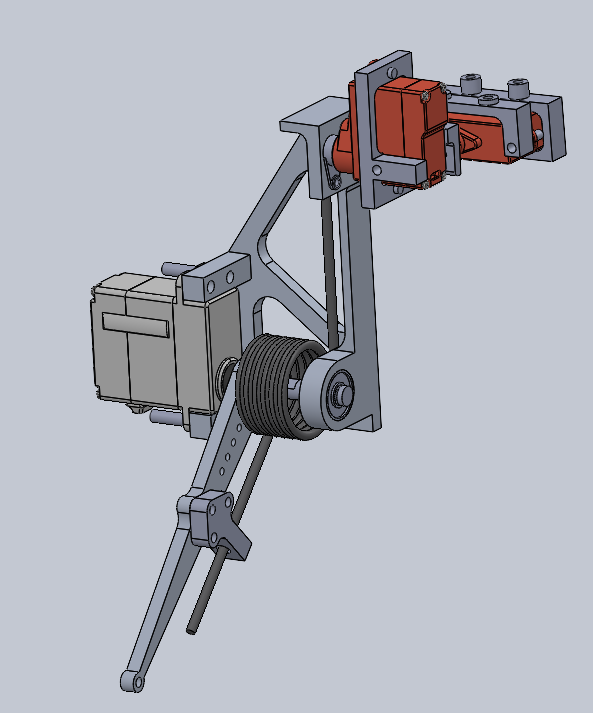
\includegraphics[width=\textwidth]{Images/CAD_leg_inside_bent.png}
        \caption{Notice the bearing holding the knee-joint shaft in place. This is important to reduce the load the motor shaft suffers in directions other than the load direction.}
        \label{fig:image1}
    \end{subfigure}
    \hfill
    \begin{subfigure}[b]{0.45\textwidth}
        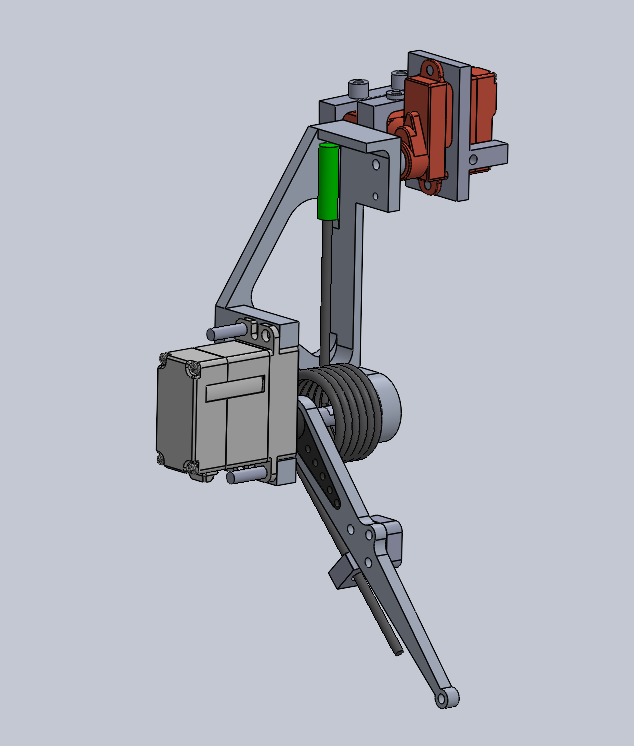
\includegraphics[width=\textwidth]{Images/CAD_leg_outside_bent.png}
        \caption{As can be seen, there is a green plastic (PLA) holster where the spring is in contact with the leg, this is to reduce  friction.}
        \label{fig:image2}
    \end{subfigure}
    \caption{An overview of the leg CAD model with a torsional spring. }
    \label{fig:assembly_CAD}
\end{figure}

\begin{figure}[h!]
    \centering
    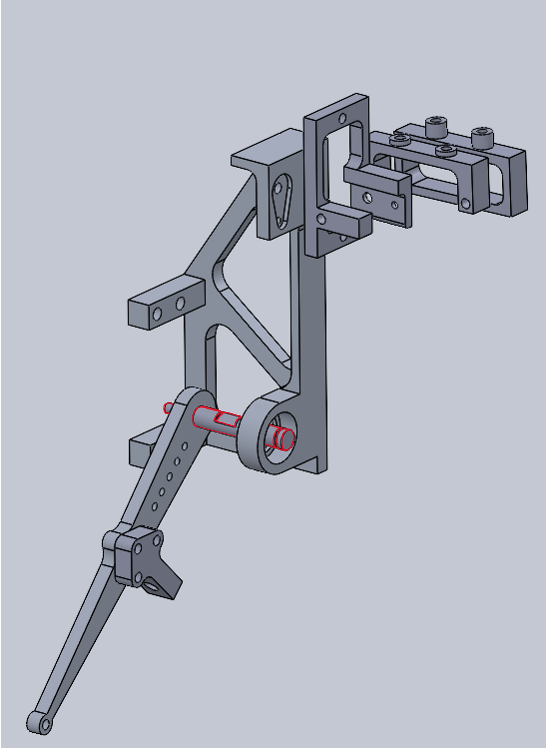
\includegraphics[width=0.6\textwidth]{Images/manufacture_only2.png}
    \caption{An overview of the CAD model of the leg design, but showing only the components that will be manufactured inhouse. Axel that will be threaded and screwed directly into the motor shaft, and lead directly into a ball bearing, is emphasized in red. }
    \label{fig:manufacture_only}
\end{figure}

\subsection{Extension Spring Leg design}
\label{sec:extension_spring_design}

The extension spring leg design is shown in figure \ref{fig:extension_spring_CAD}. As can be seen in the figure, the current design is such that the extension spring will collide with the robot shank as the knee angle approaches $\pm$ 180 degrees. Despite efforts, no solutions were found for this problem, and this design direction was therefore abandoned. Among the suggested solutions was moving the shank-end attachment point of the spring in the inwards direction, thus allowing the extension spring to lie in parallel next to the shank when the leg is fully coiled. This would however introduce a significant moment arm acting directly on the motor shaft, and this design was therefore abandoned in favor of the torsional spring design.

\begin{figure}[h!]
    \centering
    \begin{subfigure}[b]{0.45\textwidth}
        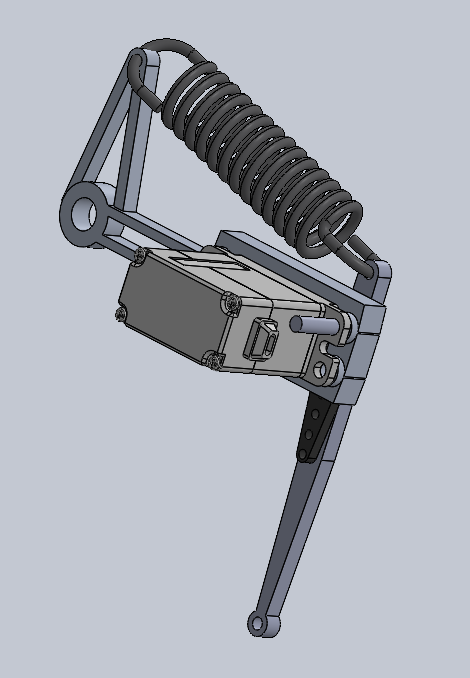
\includegraphics[width=\textwidth]{Images/extension_spring_outside.png}
        \caption{The extension spring mounted on the outside of the leg. This configuration allows for easy adjustments and replacements.}
        \label{fig:extension_spring_outside}
    \end{subfigure}
    \hfill
    \begin{subfigure}[b]{0.45\textwidth}
        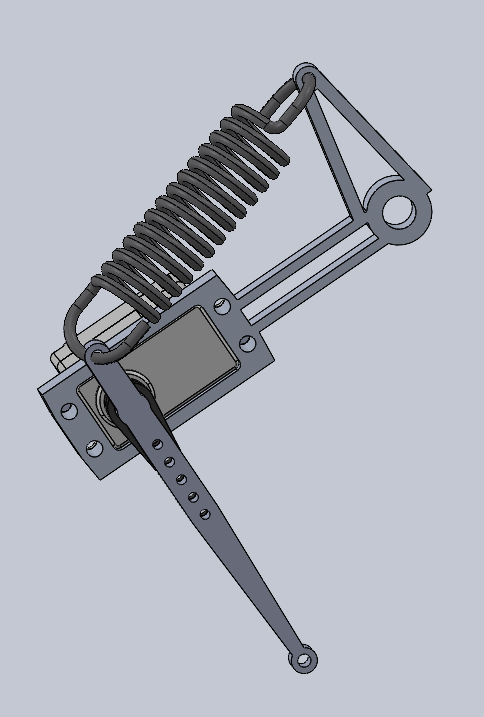
\includegraphics[width=\textwidth]{Images/extension_spring_inside.png}
        \caption{The extension spring mounted on the inside of the leg. This configuration provides a more compact design.}
        \label{fig:extension_spring_inside}
    \end{subfigure}
    \caption{Comparison of extension spring configurations: outside (left) and inside (right) the leg.}
    \label{fig:extension_spring_CAD}
\end{figure}

\subsection{Motor Selection}

As discussed in section \ref{sec:robot_design}, the choice fell on AGF-RC motors due to their high torque to weight ratio, as well as our inability to find similarly fast motors of similar strength. 

Our specific choice of motors can be found in table \ref{tab:motor_selection}. Info about the specific motors can be found in appendices \ref{appendix:A06CLS_V2_website_information} to \ref{appendix:A20_info}.

\begin{table}[h!]
    \centering
    \begin{tabular}{|c|c|}
        \hline
        Corresponding Joint & Motor Name\\ \hline
        Knee flexion/extension & A20BHM \\
        Hip flexion/extension & A06CLS V2 \\
        Hip adduction/abduction & A06CLS V2 \\ \hline
    \end{tabular}
    \caption{Selected Motors}
    \label{tab:motor_selection}
\end{table}

The reason these motors in particular were chosen is the fact that no motors were found in a similar weight class that could provide the same torque and speed. For example, if considering AGF-RC motors, the next motor, strength-wise, after the A20BHM motor, is the A35CHM motor, info about which can be found in appendix \ref{appendix:A35CHM_motor_info}. Despite being significantly heavier, the A35CHM motor is only marginally stronger than the A20BHM motor. The reasoning behind the choice of the A06CLS V2 motor was 